% Capítulo 4
\chapter{Taxonomia}
\label{cap:cap4}

Seguindo a análise dos trabalhos mencionados no Capítulo \ref{cap:cap3}, verifica-se a necessidade de classificar dos conceitos mais recorrentes atrelados ao uso do padrão \textit{throttling} em redes IoT com dirigidas energética. Além disso, é preciso levar em consideração a orientação do trabalho junto aos critérios de disponibilidade definidos por \cite{avizienis_basic_2004}, base para categorização dos elementos propostos nesta taxonomia. 

\section{Organização}

Inicialmente, as classes foram distribuídos acomodando os elementos envolvidos de acordo com os critérios que os definem, a seguir, conforme apresenta a Figura \ref{fig:taxonomia_geral}.


\begin{figure}[h]
\noindent\includegraphics[width=3cm]{example-image} 
\caption{Aqui vou colocar uma figura apresentando os dois grupos da taxonomia}
\label{fig:taxonomia_geral}
\centering
\end{figure}

Nas ramificações à esquerda, encontram-se categorias que representam as características principais relacionadas aos elementos presentes em ambientes \acf{IoT} com restrições significativas de energia. Em \cite{kansal_power_2007}  percebeu-se a necessidade de classificar estes elementos como pertencentes a uma relação de compartilhamento dos recursos disponíveis, sensores, atuadores e até mesmo os energéticos. Para isto, na taxonomia de \cite{avizienis_basic_2004} há uma divisão clara entre os agentes envolvidos e sua natureza em dois agrupamentos principais: um grupo denominado usuários ou clientes, que atua ativamente ou de forma passiva solicitando recursos ou quando notificado, consumindo os estados ofertados do segundo grupo, os provedores. Aos dispositivos provedores, cabe a responsabilidade de compartilhar seus recursos com outros consumidores através de uma interface conhecida de acordo com o protocolo de comunicação pré-estabelecido entre as partes.

Toda interação deve seguir um padrão de operação, esta é realizada de acordo com o qual se destina, como visto no trabalho de \cite{khairnar_discrete-rate_2015} é apresentado uma operação medida pela quantidade de mensagens trocadas entre dispositivos para um determinado fim. Sendo assim, os elementos classificadores encontrados são: \textit{Agentes}, \textit{Recursos} e \textit{Operações}.

Ademais, à direita, acomoda-se os elementos envolvidos no processo de adequação do comportamento de um dispositivo através da adoção do padrão \textit{Throttling}. Nesta, dois ramos principais são apresentados, \textit{Atuação} e \textit{Implementação} respectivamente. Sobre \textit{Atuação}, agrupa-se os elementos envolvidos no processo de controle do consumo dos recursos do dispositivo: \textit{Limiar} - \textit{Thresholding}, \textit{Ciclos de Carga} e \textit{Meios} estado diretamente relacionados à ação de limitar a taxa de resposta dos serviços,  \cite{khairnar_discrete-rate_2015}, \cite{khan_energy_2015} e \cite{sudevalayam_energy_2011} abordam questões que podem particularmente serem observadas para os elementos orientados energeticamente. A \textit{Implementação} é sugerida de maneira à assegurar que os critérios  \textit{Observáveis} e seus \textit{Motivadores} sejam agentes orientadores no processo de restrição às operações e incremento de disponibilidade. 


\section{Taxonomia Proposta}
A Figura\ref{label} ilustra a taxonomia proposta e os pontos abordados no processo de uso do padrão \textit{throttling} como alternativa para garantir disponibilidade nos dispositivos presentes em um ambiente  \acs{IoT} dirigida a energia. O objetivo principal é dispor os elementos ligados ao tema de maneira visual e contemplar a organização dos tópicos envolvidos. Com isso, obter:

\begin{enumerate}
    \item Visão sobre os elementos envolvidos em uma rede \acs{IoT} dirigida a energia e apresentar o \textit{Throttling} como mecanismo regulador do comportamento observando suas características energéticas;
    \item Organizar as classes de conhecimento relacionadas acomodando-as de acordo com o contexto de inserção;
    \item Suporte às definições de uso do padrão \textit{Throttling} ligados ao contexto de redes \acs{IoT} dirigida a energia. 
\end{enumerate}

\begin{figure}[h]
\noindent\includegraphics[width=3cm]{example-image} 
\caption{Aqui vou colocar uma figura da taxonomia proposta}
\label{fig:taxonomia_detalhada}
\centering
\end{figure}

A taxonomia detalhada apresenta suas classes nos termos em que foram encontrados na literatura dentro contexto de estudo, conforme Figura \ref{fig:taxonomia_detalhada}.

\section{Agentes \acs{IoT}}
Cada agente é essencialmente uma entidade que tem a capacidade intrínseca de interagir com outros agentes digitais ou físicos. Eles possuem propriedades fundamentais, como funcionalidade, desempenho, confiabilidade e segurança \cite{avizienis_basic_2004}. No contexto da Internet das Coisas (IoT), é crucial considerar sua capacidade de se comunicar com outras entidades, atuando em conjunto através do compartilhamento de recursos, características embarcadas nos dispositivos \cite{asghari_internet_2019}.


\subsection{Dispositivo Provedor}

Em qualquer instância onde um dispositivo oferece um estado ou responde a uma solicitação de recurso, ele assume o papel de provedor. Geralmente, um dispositivo desse tipo pode oferecer uma ou mais funcionalidades por meio de serviços, cada uma sendo atendida pelo uso de seus recursos enquanto avança em seus estados internos em busca de fornecer uma resposta à interação. O resultado disto será percebido como  estado externo, acessível por meio de uma interface provida na forma de eventos ou como resposta às solicitações motivadores por meio de clientes. 

Um Serviço, representa ao dispositivo provedor a forma como este lida com seus recursos embarcados. Os serviços motivam a dinâmica de mudanças de estado internos e por sua vez impactam diretamente na dinâmica de operação do dispositivo.  Por exemplo, tomemos um sistema de iluminação publica que solicita ações  a seus dispositivos encontrados dispostos em um ambiente motivados por algum evento. Assim, este sistema atua de tal forma que solicita ao dispositivo para que acione um recurso em razão de tal evento no mesmo ambiente onde o agente com capacidade de iluminação está inserido. Tal ação é ofertada pelo dispositivo via serviço que por sua vez impactará em algum desgaste dos componentes envolvidos e a utilização de seus recursos energéticos necessários.

\begin{figure}[H]
	\centering
	\caption{Representação dispositivo Provedor.}
	\label{fig:cap4bolotaprovedor}
	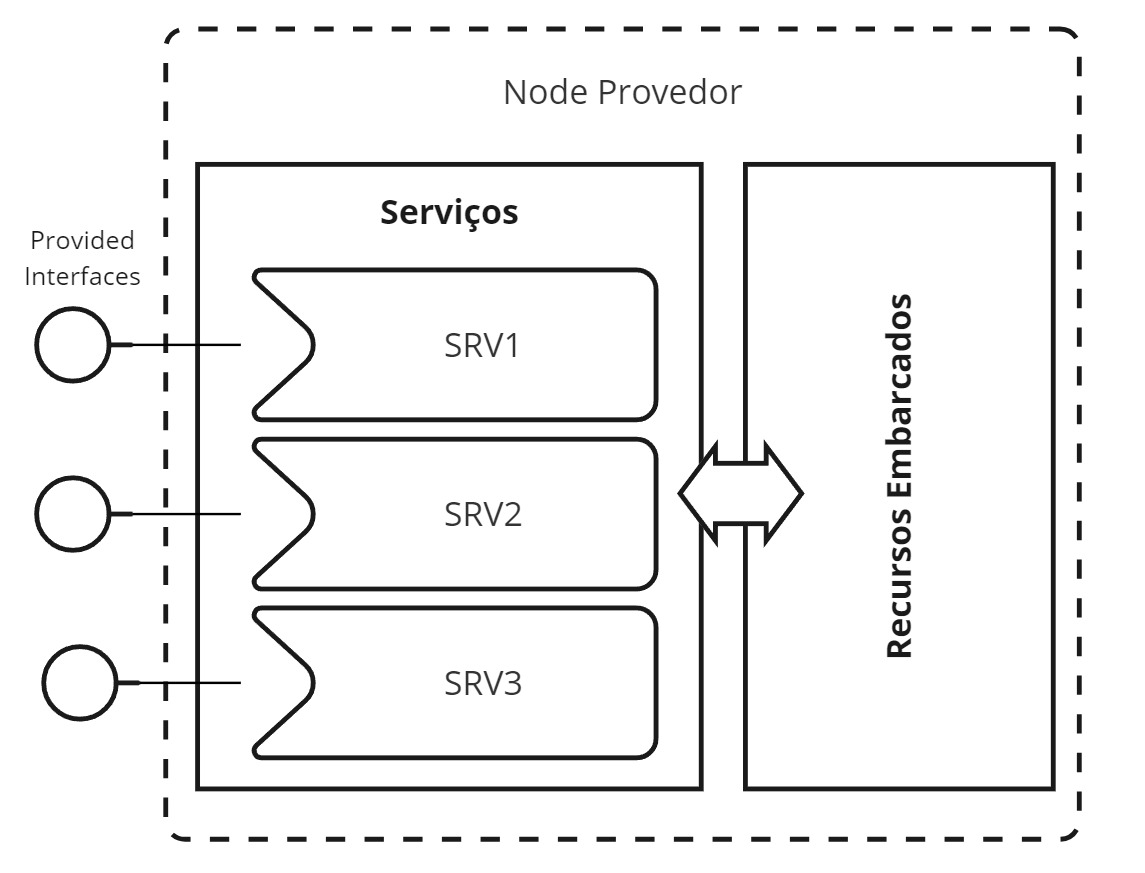
\includegraphics[width=0.7\linewidth]{Imagens/cap4/cap4nodeprovedor}	
	
	Fonte: elaborado pelo autor.
\end{figure}

\subsection{dispositivo Cliente}
Um dispositivo cliente é responsável por receber o estado externo de provedores por meio da interface disponibilizada. Ele pode consumir recursos de um ou mais provedores, dependendo da operação em execução. O dispositivo cliente comunica-se com os provedores necessários para realizar suas operações, de acordo com suas particularidades. 

\section{Operações}
Operações consiste no fluxo de mensagens comunicáveis trocadas entre dispositivos clientes e provedores. Uma operação é realizada de duas formas: quando um cliente através de mensagens solicita estado de um provedor. De outra maneira, um provedor ativamente pode disponibilizar um estado, dito externo para que um cliente possa utiliza-lo. 

Mensagem é uma unidade atômica de informação que independente do seu formato é utilizado para as mais diversas ações de acordo com o que se destina a colaboração entre dispositivos, uma mensagem pode carregar ações como  inicialização, controle, monitoramento, coleta, processamento ou armazenamento de dados. A depender da funcionalidade, um cliente quando ativo, deve enviar mensagens de solicitação aos provedores os quais reativamente respondem via interface preestabelecida, caso a operação aconteça através de eventos, o provedor deve autonomamente disponibilizará suas informações para todos que tenham interesse.

Para cobrir uma operação, múltiplas mensagens podem ser solicitadas na forma de composição de serviço \cite{service_composition}, nesse cenário um dispositivo cliente solicita mensagens distintas à um ou vários dispositivos provedores para compor este serviço. Em todo caso, como encontrado na revisão \cite{kahloul_service_2019} a abordagem das operações encontrada nos serviços puramente virtuais não acomodam por completo a natureza operacional dos agentes \acp{IoT}. Para tal, precisa-se considerar o modo de operação dos dispositivos, seus estados e recursos pois se encontram diretamente em um meio físico e precisam lidar com as particularidades inerentes a um ambiente dinâmico e seus desafios.

\section{Recursos Energéticos}

Um Recurso descreve um componente ou capacidade que um dispositivo possui para realizar suas operações. Isto inclui seus componentes físicos ou virtuais que uma vez embarcados ao dispositivo contribuem em cooperação para os mais diversos fins, coleta, monitoramento, automação industrial, assistência a medicina entre outros. Um Recurso infere sobre as capacidades dos elementos dispostos na rede, a configuração do dispositivo esta fortemente ligado à atividade fim que se destina. Para esta taxonomia, características como capacidade de processamento, armazenamento ou transmissão de dados estão omitidos pois expressam diretamente o universo de possibilidades onde um agente \acs{IoT} se encontra. Entretanto, em uma rede \acp{IoT} dirigida à energia, aspectos energéticos devem ser detalhados.

Recursos energéticos, por sua vez refere-se a dois grupos: da capacidade de coleta do dispositivo e a da capacidade de armazenamento e disponibilização dessa energia previamente coletada. Arquitetura de sistemas dirigidos a energia com capacidade de coleta são projetados para usar recursos energéticos de maneira eficiente como descrito em \cite{prauzek_energy_2018} sua aplicação é especialmente útil em cenários onde a energia para alimentar os dispositivos é escassa. Um recurso energético é uma fonte natural ou artificial de energia que apropriadamente pode ser convertida em energia utilizável suplementando as necessidades para realizar operações.

No cenário proposto, observar esses recursos energéticos assume um papel importante pois é essencial para garantir o funcionamento continuo e autônomo dos dispositivos envolvidos, cabendo ao agente embarcado suas ações de coleta, transformação, armazenamento e utilização o recurso energético, projetado de maneira a capacitar o dispositivo a operar enquanto busca um cenário de neutralidade energética.

% \subsection{Sensores}
% Um sensor é um recurso capaz de detectar e medir informações específicas do ambiente ao redor. Convertendo características do meio físico como temperatura, umidade, luz, pressão, movimento, som em sinais digitais que podem ser processados. 

% \subsection{Atuadores}
% Por sua vez, um atuador é um componente que converte um sinal de entrada em um movimento físico ou ação. Em um sistema de controle um atuador pode receber uma entrada provida por um sensor e agir em detrimento do estimulo capturado.  Atuadores geralmente são categorizados em: elétricos, hidráulicos, pneumáticos, mecânicos (por exemplo, atuadores de engrenagens), magnéticos, piezoelétricos entre outros.





\subsection{Capacidade de Coleta}\label{Capacidade de Coleta}
De acordo com o trabalho de \cite{sudevalayam_energy_2011}, a capacidade de coleta refere-se à habilidade do elemento em extrair e transformar um recurso energético disponível no ambiente. Seu objetivo é manter ou estender o tempo de funcionamento do dispositivo, atendendo totalmente ou parcialmente às suas necessidades energéticas.

Sistemas de coleta energética possuem três conceitos fundamentais: Carga, a Arquitetura de Coleta e entrada energética. A Carga é destinada a atividade que esta consumindo energia, este é oriundo de um componente demandante de energia para operar, sejam sensores, transmissores ou  atuadores, apresentados como uma composição de recursos. A Arquitetura de Coleta indica quais mecanismos, deve descrever seus componentes, meios de conversão e unidades de armazenamento. Atualmente é possível destacar três modelos básicos de arquitetura:

\begin{itemize}
    \item Coleta e Usa (\textit{Harvest-Use}): Neste modelo, toda energia coletada é oferecida diretamente ao dispositivo continuamente. Conforme \cite{merrett_energy-driven_2017}, um dispositivo não precisaria de um \textit{buffer} energético, desde que seu funcionamento fosse orientado as características \textit{Power-Neutral}. Assim, a energia coletada deve satisfazer os valores de operação plena ou pelo menos o minimo necessário para o funcionamento depreciado. Assim, caso a energia coletada não seja suficiente, o dispositivo prontamente adaptará o fornecimento dos seus recursos buscando enquadrar-se a disponibilidade energética corrente para, posteriormente, caso o nível de fornecimento energético se restabeleça, tenha sua operação normalizada. Em alguns casos, quando prontamente é detectado níveis energéticos abaixo do necessário até para o funcionamento circunstanciado do dispositivo, é possível com alguma antecipação do cenário realizar rotina que vise preservar seu estado mediante criação de \textit{checkpoints}, assim restabelecida as condições energéticas, retornar para um estado desejado, característica de um sistema intermitente apresentado por \citeauthor{sliper_energy-driven_2020} (\citeyear{sliper_energy-driven_2020}).
    
	\begin{figure}[h]
			\centering
			\noindent\includegraphics[width=3cm]{example-image} 
			\caption{Aqui vou colocar uma figura power-neutral}	
	\end{figure}   
    
    \item Coleta, Armazena e Usa (\textit{Harvest-Store Use}): Dispositivos inseridos em um dado ambiente coletam energia do meio para seu uso. Todavia, precisam lidar com o dinamismo da natureza energética coletada, embarca-se a capacidade de armazenar energia coletada em um \textit{buffer} e assim, disponibilizar esta entrada para uso nos ciclos do dispositivo. Este modelo tem objetivo reduzir problemas derivados da variação do montante energético coletado pelo \acs{EHS}, seja pela momentaneamente pela escassez de energia disponível ou depreciação do modelo de coleta.
    
    \begin{figure}[h]
    	\centering
    	\noindent\includegraphics[width=3cm]{example-image} 
    	\caption{Aqui vou colocar uma figura energy-neutral}	
   	\end{figure}  
    
\end{itemize}


A depender da especificidade dos ambientes onde os dispositivos se encontram, técnicas podem ser utilizadas para a extração de energia disponível, a conversão de fontes renováveis solar e eólica, a captura da força \textit{piezo-elétrica}, termodinâmica, entre outros. A adequação da estratégia de coleta e seus detalhes devem ser projetados de acordo com o meio, capacidade do dispositivo e a natureza da fonte energética que objetiva-se coletar. Em geral, a divisão das características dos ambientes já descrito em \cite{shaikh_energy_2016} é referencia utilizada para categoriza-las de acordo com seus ambientes, assim a analisar as características das fontes energéticas, temos:

\begin{itemize}

    \item Não controladas mas previsíveis: A produção energética não pode ser controlada nos momentos desejados, mas o comportamento pode ser modelado para prever a disponibilidade num dado momento com alguma margem de acerto. Por exemplo, no trabalho de  \cite{lee_energy_2018} fontes energéticas baseadas em energia energia solar, que tem sua origem não controladas, todavia existem modelos capazes de prever  disponibilidade energética para colheita de acordo com sua sazonalidade durante ciclos diurnos.
    
    \item Não controladas e não previsíveis: A fonte energética não pode ser controlada para gerar energia quando desejado e não é fácil prever usando um modelo quando será possível. A extração energética originada pela vibração de ambientes internos é um exemplo de tal fonte energética como descrito em \cite{wei_comprehensive_2017}, todavia definir padrões de sazonalidade das vibrações pode tornar o processo de coleta impraticável;
    
    \item Completamente controlada: Neste contexto, a energia é gerada apenas quando necessário, como visto em alguns sistemas \textit{piezoelétrico} onde através da interação humana para geram energia quando necessário.
    
    \item Parcialmente controlada: O processo de geração energética é sensível à ação de terceiros porém a quantidade exata de energia gerada não pode ser prevista com exatidão. Fontes baseadas em Radio Frequência converte a transmissão de ondas de radio em energia utilizável, por exemplo, \cite{shaikh_energy_2016} decorre como tags \acf{RFID} conseguem ser visualizadas por um leitor. Todavia, a quantidade de energia coletada sofre impactos diretos das características de propagação no meio disposto, barreira, distancia até a fonte e capacidade da antena de transmissão.
\end{itemize}

\subsection{Capacidade de Armazenamento}\label{Capacidade de Armazenamento}
A capacidade de armazenamento trata das propriedades como conversão, força e taxa de carregamento e descarga em relação a fonte energética em uso com o objetivo de utilizar essa energia em momento apropriado. 

É bem conhecido que o fator energético é um desafio para dispositivos com restrições energéticas e capacidade de coleta, pois claramente caso o recurso energético deste seja esgotado o mesmo não será capaz de cumprir seu papel, sob a condição do restabelecimento deste recurso ou algum mecanismo de armazenamento possa cobrir parcial ou totalmente a diferença energética necessária para a operação.

Baterias, super capacitores ou modelos híbridos estão presentes no contexto de dispositivos com fortes restrições energéticas e capacidade de coleta, para estes a atuação busca estar de acordo com as condições físicas e necessidade de conservação da energia na forma de conceber este \textit{buffer} denominado \textit{Storage}. É possível distinguir dois padrões de armazenamento para as capacidade energética presente em um dispositivo que busca observar a relação entre a saída energética e o gasto energético do dispositivo. Segundo o modelo, a habilidade para coletar e a necessidade de disponibilidade devem ser definidas em um acordo de serviço \acs{SLA}. Portanto, um dispositivo deve ter sua capacidade de armazenamento definida em:

\begin{itemize}
    \item dispositivo provedor sem \textit{Storage}: Aqui não existe a necessidade estrita da gestão de recursos elétricos pois caso não exista energia suficiente o dispositivo poderá adaptar-se na tentativa de alinhar a necessidade energética ao fornecido no momento, em outros casos, sua operação se assemelhará a operação transientes ja caraterizado por  \citeauthor{sliper_energy-driven_2020} (\citeyear{sliper_energy-driven_2020}), preparados para interromper suas atividades e, ao restabelecer sua entrada energética disponível, retornar a partir de um ponto previamente estabelecido (\textit{checkpoint}). 
    
    \item dispositivo provedor com \textit{Storage}: Neste caso, um dispositivo carrega em si a capacidade de armazenar energia coletada em um \textit{buffer}. A gestão energética deve ocorrer para que a energia coletada seja previamente armazenada para assim, ser disponibilizada em ciclos. Aqui os dispositivos operam em um regime de Coleta, Armazenamento e Uso.
\end{itemize}

\section{\textit{Throttling}}

Aplicar o padrão \textit{Throttling} consiste basicamente em restringir o uso de recursos de acordo com limiares de utilização estabelecidos. Seu objetivo é proteger um dispositivo do estado de sobrecarga, evitando que consumidores excessivamente solicitantes coloquem um dispositivo provedor em um estado de sobrecarga, evitando possíveis falhas e a exaustão prematura de recursos \cite{martinekuan_throttling_nodate}. Com isso, a estratégia permite que provedores consigam operar dentro de termos definidos por um acordo de funcionamento conhecido como \acf{SLA}, protegendo este provedor de assumir um estado de sobrecarga onde precise atender mais solicitações do que o adequado para sua capacidade.

Na taxonomia, o uso do \textit{Throttling} é candidato à colaborar nas atividades que buscam aumentar disponibilidade do provedor, conservando  recursos energéticos e suas observações a respeito de características ou limitações do próprio dispositivo. Para tal, é preciso que limiares sejam estritamente adequados ao que se aplica, capacidade de transmissão, recursos disponíveis ou esperados pelo dispositivo. Definir limiares de operação realísticos que atendam as necessidades de um dispositivo provedor é um desafio relevante para sistemas com estratégia de coleta de energia \cite{khairnar_discrete-rate_2015}, \cite{liu_energy_2016} e \cite{zhang_toward_2018}, entregando capacidade de decisão sobre as atidades realizadas nos ciclos enquanto se objetiva conservar-se.

\subsection{Atuação: Limiar, Ciclo de Carga, Observáveis e Meios}
\label{cap4:atuação}
Em sistemas \acs{IoT} orientados aos fatores energéticos, a atuação do padrão é dada ao monitorar a taxa de solicitações no decorrer de um espaço de tempo, nesse intervalo, denominado Ciclo de Carga. Durante um ciclo clientes podem fazer requisições ao dispositivo provedor. Do ponto de vista da disponibilização dos recursos, durante um ciclo de carga, um dispositivo pode assumir abordagem de equidade entre os solicitantes ou algum critério de prioridade e privilégio, onde um solicitante qualquer teria suas requisições atendidas mediante negação do serviço para outro cliente com menor prioridade, caso necessário.

Uma vez definido um limiar de atuação, sua ação pode ser constante durante todo funcionamento do dispositivo, assim o mesmo valor limiar é aplicado independente de outros fatores, outra possibilidade é definir vários limiares que agem adaptativamente de acordo com os modos de operação mapeados, tão logo determinado cenário seja alcançado, o dispositivo pode ajustar seu limiar de atuação para conservar seus recursos visando manter-se funcional. O comportamento do limiar de atuação passa pela analise cuidadosa da natureza das operações esperadas para o dispositivo. Em síntese:

\begin{itemize}
    \item Limiar constante: Seu valor é fixado e estabelecido enquanto o dispositivo é projetado. Este limiar pode ser determinado considerando fatores como testes de desempenho, características do ambiente onde será inserido e requisitos operacionais. Todavia, uma vez definido, o limiar permanecerá constante ao longo de todo o momento em que  atividades são realizadas.
    
    Por exemplo, considere um dispositivo com uma dada capacidade de processar mensagens, este pode estabelecer um limiar constante para o máximo de requisições processáveis simultaneamente. Sendo assim, em toda operação, caso esse limiar de requisições seja atingido, irá ativamente rejeitar ou atrasar o atendimento das solicitações de serviço até que o valor de requisições retorne ao nível aceitado. 
    
    Esta abordagem, é bastante útil caso se conheça bem as capacidades do dispositivo e não se espera uma grande variação nas condições de operação ao longo do tempo. Embora oferte equidade do ponto de vista dos solicitantes, que tem suas requisições atendidas segundo os mesmos critérios independente do estado do dispositivo provedor, não é garantido que uso dos recursos será adequado caso ocorra mudanças repentinas ou flutuações significativas nos termos de funcionamento deste provedor.
    
    \item Limiar adaptável: Nesta abordagem, o comportamento do dispositivo é ajustado dinamicamente, por isso pode assumir um comportamento mais adequado ao observar suas condições de funcionamento através do monitoramento ou análise dos seus recursos. Permitindo atender as solicitações dos clientes, com performance adequada aos termos de operação que se encontre. Por exemplo, dado um sistema de segurança que geralmente possui dispositivos equipados com câmeras. Este provedor, deve enviar imagens capturadas por seus sensores para algum solicitante, seja uma central que passivamente recebe as gravações ou outra forma de demandante devidamente conhecido. Seja uma mudança observada em seus termos de funcionamento, o dispositivo poderá ter faixas de limiares distintas adequando-se ao estado encontrado, por exemplo, operações diurnas ou noturnas, conservando-se e garantido seu funcionamento dentro do acordo de serviço estabelecido.   
    
    \begin{figure}[h]
    	\centering
    	\includegraphics[width=3cm]{example-image} 
    	\caption{Aqui vou colocar uma figura A e B com as diferentes atuações do limiar.}
    \end{figure}
    
    
\end{itemize}

Graças a isso, o dispositivo com limiares de atuação adaptáveis será capaz de adequar seu modo de operação em diferentes zonas de uso, depreciando seus serviços como mudança de comportamento, seja para interromper ou reduzir sua taxa da transmissão, aumentando seu tempo de inatividade e assim mitigar riscos funcionais enquanto se encontra em um modo mais ou menos parcialmente restrito. Uma vez que os recursos energéticos observáveis se restabeleçam, pode-se assumir um comportamento de uso que acentua o uso dos recursos disponíveis, incentivado pelo novo valor estipulado para o limiar de consumo. Esta capacidade de adaptação, permite que dispositivos mantenham algum equilíbrio entre conservação de recursos e performance, sustentado pela adaptação promovida pelos modos de operação definidos, garantindo suas funcionalidades em termos das condições operacionais.


Qualquer aspecto que impacte ou influencie na capacidade do dispositivo em manter-se disponível deve ser considerado em sua atuação. Estes, ditos elementos observáveis, compreendem os componentes aos quais cabem a analise de estado, pois justificam a ação do mecanismo throttling, que deverá indicar o comportamento do dispositivo para mante-lo adequado mediante evitar seu esgotamento energético. Para tal, se apresentam como os garantidores das condições energéticas do dispositivo: sua condição de entrada através de uma fonte energética; a capacidade de armazenamento dessa energia coletada em eventual \textit{buffer}. 

\subsubsection{Meios}
\label{cap4:atuacao_meios}
O comportamento de um dispositivo pode ser ajustado de acordo com as circunstâncias. Diferentes meios são usados no processo de construção do mecanismo \textit{throttling} a depender das características de atuação do dispositivo executará e a intenção particular ao limitar suas operações. Assim, os meios de atuação decorrem sobre:

\begin{itemize}
	\item Meio 1: Atuação sobre dispositivos clientes; 
	\item Meio 2:\label{meio2} Atuação sobre atividades do dispositivos provedor;
	\item Meio 3:\label{meio3} Atuação sobre degradação intencional de componentes envolvidos.
\end{itemize}

O Meio 1 utiliza os mecanismos de throttling ao considerar a necessidade de observar as capacidades dos clientes em relação de sua taxa de vazão ou a criticidade de suas operações. Sobre a taxa de vazão, espera que o limitador aplicado atue sobre a taxa de recebimento das mensagens em acordo com a capacidade e suas restrições para lidar com tais eventos. Sendo assim, o dispositivo cliente poderá limitar sua vazão para envio de novas solicitações ou a sua disponibilidade para recebimento de novas informações de acordo com o modo de operação encontrado em decorrência das capacidades observadas que classificam o modo.

Entende-se por criticidade de um cliente, o atributo que indica fundamentalmente a importância das operações realizadas por este dispositivo em detrimento as consequências da não realização de uma operação dita critica. Assim, é previsto dois cenários: um primeiro onde todas as operações tem igual importância para este dispositivo, e um segundo, onde existam operações classificadas mais importantes ou criticas que outras. Sendo assim, de acordo com o segundo cenário, justifica-se que tais operações possam encontrar um cenário com limiar de \textit{throttling} aliviado e por isso, cabe observar e definir tais valores para que dado aconteça operações privilégiadas, exista também a justificativa de maior tolerância quanto ao uso de recursos para o cumprimento destas. 

Certamente, para que seja possível um maior gasto de recursos pelas operações criticas, cabe também ao projeto definir regras de compensação onde caso necessário, o dispositivo poderá reduzir seu limiar para outras demandas, motivados a preservar parte do seus recursos que em outro momento seria utilizado por estas demandas menos privilegiadas.

Meio 2 compreende o controle de atuação no dispositivo provedor. De acordo com o seu estado durante um ciclo os mecanismos de throttling poderão atuar em conformidade aos recursos encontrados. Para tal, as estratégias de aplicação e definição de limiares passam pela observação da capacidade de vazão das múltiplas solicitações proveniente dos clientes, bem como da criticidade das operações realizadas. 

A taxa de vazão do um dispositivo provedor, é definida pela sua capacidade em atender demandas dos diversos solicitantes durante um espaço de tempo, seja por limitação de transmissão ou por sua capacidade computacional em realizar tais operações ou mesmo seu modo de operação definidos em relação aos recursos energéticos. Sendo assim, o mecanismo de throttling poderá se valer dos limiares estipulados através da análise dos recursos para operação e, a partir daí, dado o cenário encontrado, limitar o atendimento as solicitações de solicitantes considerados excessivamente demandantes ou menos privilégiados.  

Quanto a observação das operações realizadas pelo dispositivo provedor, estas tem seu grau de criticidade atrelado a importância de tal operação na conjuntura ao que se destina o dispositivo. É importante destacar que a definição de limiares sempre busca garantir que o dispositivo não consuma seus recursos de maneira desnecessária, aqui considerado um gasto excessivo. O Limiar de atuação deveria ser revisto idealmente a todo momento que o panorama encontrado pelo dispositivo mude, seja pelo fim de um ciclo de atividades ou a medida que solicitantes sejam atendidos. Com isso, dado limiar deverá atuar protegendo o dispositivo provedor no decorrer de sua mudança de estado ao passo que realiza as operações. 

O limiar de atendimento de operações poderá suportar um sistema hierárquico, similar ao já definido sobre a criticidade das operações dos dispositivos clientes. Neste caso, é de conhecimento do dispositivo provedor quais solicitantes privilégiados terão suas operações realizadas mesmo em um cenário mais restrito, outro ponto é que dado a criticidade da operação pode-se fazer distinções, tolerando mais operações de um tipo considerado privilégiado.

Pode-se ainda, anexar ao conjunto relacionado aos fatores utilizados para definição do limiar das operações, os aspectos ligados a degradação ativa nos componentes envolvidos nas operações ofertadas ou apenas de uso interno do dispositivo. Ao limitar alguma operação, apresenta-se a oportunidade para que o \textit{throttling} no dispositivo também possa restringir o uso de recurso energético de algum componente inativo, neste caso, cercear parcial ou totalmente a utilização energética dos componentes envolvidos com tais operações limitadas. 

Compreende os mecanismos dispostos no Meio 3, a capacidade do nó em reduzir o consumo energético de algum componente embarcado mediante o cenário de escassez energética. Esta já é uma manobra conhecida; diversos dispositivos submetem-se a esta, objetivando a conservação de seus recursos energéticos durante ciclos, especialmente quando não existe uma previsibilidade de uma nova oferta energética. Por exemplo, os aparelhos móveis possuem a capacidade para que, dado limiar de  sua reserva energética (\textit{Storage}) seja atingido, limita-se ativamente os componentes menos críticos, por exemplo câmeras de alta definição ou alto-falantes, assim, o recurso energético usado por tais pode ser conservado e disponibilizado para componentes dito essenciais até que o cenário de escassez se resolva. 


\subsection{Motivadores}

Além das operações realizadas, a implementação do padrão throttling passa por avaliar os agentes que impactam diretamente o comportamento do dispositivo. Este, também deve considerar a atuação do mesmo enquanto dispositivo \acs{IoT}. 

A entrada energética em \ref{Capacidade de Coleta}, indica a capacidade do dispositivo em captar recursos energéticos através de um mecanismo de coleta, uma vez que um dispositivo receba esta entrada, dará inicio um novo ciclos que por sua vez durará até a próxima oferta energética. Sobre a capacidade de armazenar energia, como decorrido em \ref{Capacidade de Armazenamento} indica sua reserva energética (\textit{Storage}) onde, em momento adequado, poderá fazer uso para manter-se operacional.  

A capacidade do dispositivo em entender a dinâmica dos fatores que interagem com os valores coletados na forma de entrada energética através do seu \textit{Power Supply} e reserva (\textit{Storage}) é fundamental para garantir maior disponibilidade. Estes fatores compreende os observáveis, grupo motivador do ajuste de comportamento dos mecanismos providos pela atuação do \textit{throttling}. 

Desta forma, a mudança de comportamento do dispositivo motiva-se em: tão logo os fatores de tomada de decisão forem alcançados, adequar-se para que estes fatores agora considerados divergentes, sejam superados motivados pela mudança de modo de operação buscando retornar ao cenário que representa as capacidades de atendimento do dispositivo.   Por isso, o agente limitador deve agir de maneira suficientemente rápida para que a mudança de estados seja alcançada o mais brevemente possível, referente à capacidade do dispositivo em dispender recursos para realizar operações. 

No trabalho \cite{zhang_toward_2018}, equipamentos capazes de observar seus recursos energéticos, atuam modificando seu comportamento para preservar energia motivados com a expectativa de uma entrada energética prevista. Sendo assim, para este caso, a motivação de aplicação do agente limitante é preservar alguma condição energética, prolongando a disponibilidade dos componentes ditos críticos. Portanto, a motivação dos dispositivos em limitar seu comportamento passa pela análise do estado dos recursos observáveis e a intenção que se deseja alcançar em acordo com agente limitante.

Assim, caso um limiar de atuação seja atingido a alteração de comportamento precisa ocorrer de modo adequado, mitigando, com isso, perdas desnecessárias ou não previstas, causadas por ajuste inapropriados de comportamento. Considerando que o ajuste demorado potencialmente coloca o dispositivo em não ter um modo de operação adequando às suas condições reais.


Para justificar a atuação dos mecanismos de limitação, é preciso definir quais os motivadores, Sendo estes o propósito declarado para restringir operações em concordância com a causa motivadora. Assim, é de interesse dos aspectos relativos a considerações das capacidades energéticas do dispositivo, que a atuação do \textit{throttling} procure alcançar um dos dois objetivos, sendo estes os motivadores:

\begin{enumerate}
	\item Preservar recursos energéticos. 
	Evitar gasto excessivo ou inadequado é primeiro motivador de um agente limitante embarcado em dispositivos com restrições energéticas, pretende-se com isso manter o dispositivo em um estado adequado em relação das capacidades energéticas dispendendo recursos de maneira inferior ou próximos a zona neutro-energética onde a energia coletada é suficiente para todas operações realizadas na duração do ciclos de carga.
	
	\item Restabelecimento da condição energética.
	Quanto a recuperar seus recursos energéticos, entende-se que o dispositivo poderá através da analise de seus observáveis, adotar comportamento limitado motivado pela expectativa de restabelecer seus recursos energéticos a valores esperados. Neste caso, pretende-se com isso manter-se em modo de operação que favoreça dispender menos energia durante os próximos ciclos de carga até que seus recursos observáveis retornem em acordo com o esperado ou seu cenário de uso seja alterado. Uma vez alcançado um estado desejado, o dispositivo poderá reavaliar seu comportamento e ajustar-se para o modo de operação considerado adequado. 
\end{enumerate}





\begin{comment}
	
estão dispostos em cenário de disponibilidade energética previsível onde é necessário em prever a quantidade futura de energia coletável disponível para recarga. O problema foi apresentado na forma de um \ac{MDP} onde os dispositivos podem adequar seu comportamento de acordo com expectativa energética vindoura para recarga. 


acima do que de fato deveriam Ocasionando até mesmo, um cenário de maior esgotamento energético do que previso

coloque o agente em um modo de operação inadequado, fora do esperado. A depender de como as operações ocorrem, o modo de operação terá capacidade de criar um cenário de esgotamento energético acelerado, em outra parte, a limitação inapropriada poderá causar sobrecarga de atividades para outros elementos da rede, por exemplo.
	

Estes aspecto podem ter seus valores pré-estabelecidos, porém é comum enfrentar situações onde os valores tidos como justificadores de um comportamento não sejam suficientemente adequados, seja por uma falha na previsibilidade de um recurso ou evento não tolerável. Por exemplo, é relativamente comum um cenário onde dispositivos que exploram energia solar diurnalmente enfrentem alguma escassez energética motivados por eventos climáticos não previstos. Com isso, colocam em risco sua disponibilidade, pois caso seja mantido o comportamento dito adequado e previamente estabelecido podem levar o dispositivo a um alterações em sua disponibilidade não previstas ou perdas em performance. 

No contexto de dispositivos com capacidade de coleta energética, fatores pré-estabelecidos são comumente encontrados, ciclos de recarga na forma de capacidade de coleta, a capacidade de armazenamento do dispositivo e a sazonalidade da fonte energética coletável. O conjunto dos valores  desses fatores presentes no dispositivo, indicam o estado energético deste agente. Dado um estado energético esperado, pode-se previamente definir como o dispositivo se comportará. Mesmo assim, também vale ressaltar que estes elementos energéticos estão relacionados às variações e toda sorte de situações que o dispositivo provedor enfrenta enquanto agente em campo. Diversos esforços foram realizados para melhorar a maneira como um agente observa seu estado energético e define seu comportamento, mas para que seja possível adequar-se concretamente à estes fatores encontrados, o agente deve ter a capacidade de analisar as operações e o cenário onde se encontra, tanto individualmente quanto, se possível, em conjunto com outros elementos colaboradores. Assim, é possível realizar ajustes prontamente nos limiares de atuação, tão logo perceba-se que os valores estimados previamente e o seu estado esperado divirjam causando comportamento fora do desejado.

\end{comment}  









